

\ifdefined\maindoc
% \graphicspath is additive (appends, does not replace), so this adds this chapter's own
% figures folder to whatever main.tex's own \graphicspath already lists, regardless of whether
% that centralized list has been kept up to date. Real folder per main.tex's own \include line:
% Chapters/Introduction/figures/.
\graphicspath{{Chapters/Introduction/figures/}}
\else
\documentclass[12pt]{report}
\usepackage[a4paper,margin=1in]{geometry}
\usepackage[utf8]{inputenc}
\usepackage[T1]{fontenc}
\usepackage{amsmath,amssymb}
\usepackage{booktabs}
\usepackage{setspace}
\usepackage{graphicx}
\usepackage{enumitem}
\usepackage{placeins}
\usepackage{hyperref}
\usepackage{array}
\usepackage[backend=biber,style=ieee,citestyle=numeric-comp,sorting=none]{biblatex}
\addbibresource{references.bib}
\setcounter{biburllcpenalty}{7000}
\setcounter{biburlucpenalty}{8000}
\setcounter{biburlnumpenalty}{9000}
\onehalfspacing
\graphicspath{{figures/}}
% Standalone-only fallbacks so Chapter~\ref{...} renders as the right number outside the
% main thesis. Under \maindoc these are skipped and the real labels in main.tex resolve.
% Numbers per the confirmed live chapter order (Overleaf compile log, 2026-08-25): 1 this
% chapter, 2 Background, 3 Network Model, 4 Input Module, 5 Diamond, 6 Probability, 7 Capacity,
% 8 CPM, 9 Julia package, 10 Front End, 11 Integrated Case Study.
\makeatletter
\newlabel{ch:lit-review}{{2}{1}{}{Doc-Start}{}}
\newlabel{ch:system-model}{{3}{1}{}{Doc-Start}{}}
\newlabel{ch:input-module}{{4}{1}{}{Doc-Start}{}}
\newlabel{ch:diamond-module}{{5}{1}{}{Doc-Start}{}}
\newlabel{ch:probability-toolkit}{{6}{1}{}{Doc-Start}{}}
\newlabel{ch:capacity-toolkit}{{7}{1}{}{Doc-Start}{}}
\newlabel{ch:critical-path}{{8}{1}{}{Doc-Start}{}}
\newlabel{ch:julia-package}{{9}{1}{}{Doc-Start}{}}
\newlabel{ch:front-end}{{10}{1}{}{Doc-Start}{}}
\newlabel{ch:integrated-case-study}{{11}{1}{}{Doc-Start}{}}
\makeatother
\begin{document}
\title{Introduction}
\fi

\section{Motivation}
\label{sec:intro-motivation}

A water distribution network, a power grid, a plant process line and a construction schedule are
frequently the same kind of directed dependency structure, asked three different questions: does
the system keep functioning when a component fails, how much can it carry, and when does a
dependent sequence of activities finish. Reliability computation, flow analysis and schedule
analysis answer these three questions separately, each with its own methods, and each typically
consuming a single precise number for what it does not know exactly about its inputs, a component
failure probability, an edge capacity, an activity duration.

No tool or method combines all three of these analyses on one network with any of them
propagating interval or probability-box uncertainty natively. Huang, Huang and Lin's exact
project-reliability method pairs reliability with schedule but not flow, computing the probability
that a project completes within both a time and a budget constraint from discrete, point-valued
activity states \cite{huang2020exact}. Tong's Georgia Tech dissertation pairs reliability with
flow but not schedule, using a point-valued probability propagation method throughout
\cite{tong2021infrastructure}. Running several kinds of analysis against one shared network object
is itself not new: \texttt{pandapower}, an open-source power-system tool, runs five different
analyses, power flow, optimal power flow, state estimation, topological search and short-circuit
calculation, against one shared graph of buses and lines \cite{thurner2018pandapower}. None of
these three, and nothing else found in a systematic search, combines reachability reliability,
capacitated flow and activity scheduling on one network representation with native imprecision
propagation across the combination. Chapter~\ref{ch:lit-review} surveys this landscape in full.

This thesis develops a framework that closes that gap: one network representation supporting all
three analyses, native interval and probability-box propagation wherever the underlying
computation supports it, and delivery through a local, no-code interface rather than a script.
Figure~\ref{fig:intro-framework-overview} sketches the framework this way, top to bottom: the
network representation and its decomposition strategy, the propagation algorithms the three
toolkits share a common structure through, the point at which each toolkit's imprecision support
actually stops, reliability carrying intervals and probability boxes, schedule carrying intervals
only, flow carrying neither yet, and the package and interface the whole framework is delivered
through.

\begin{figure}[htbp]
  \centering
  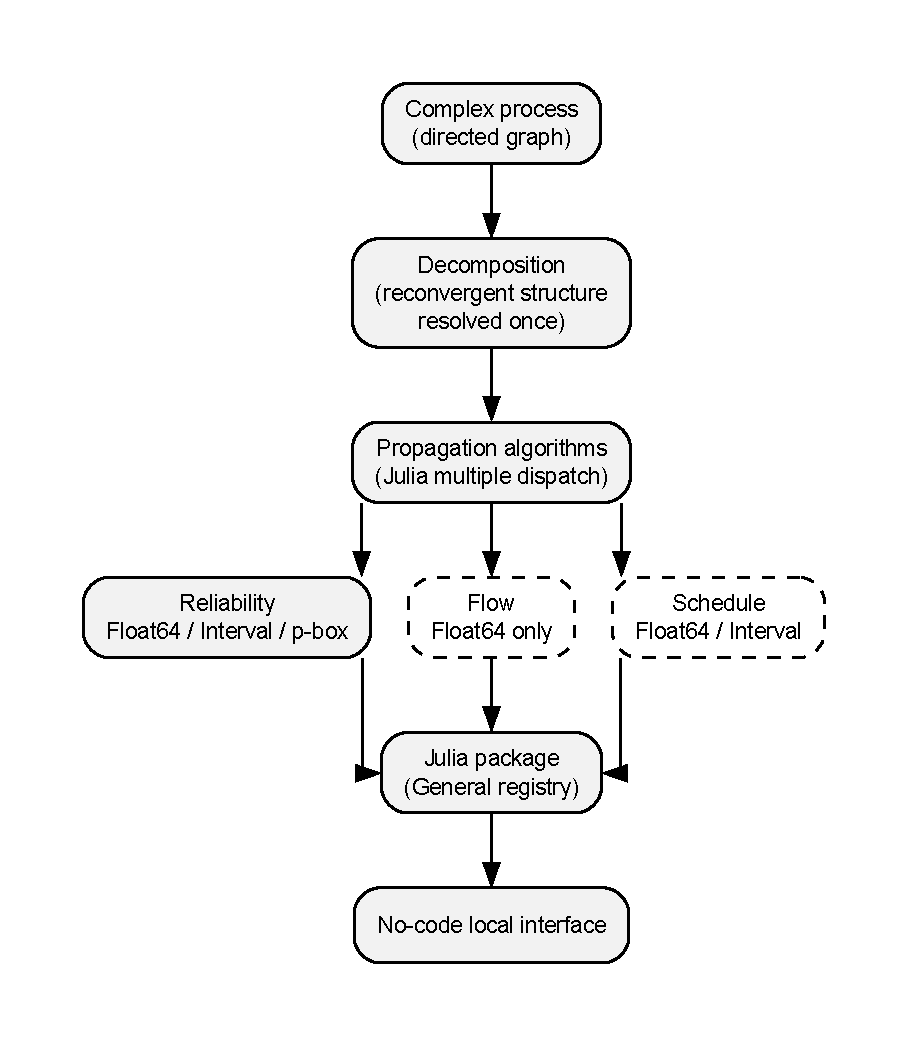
\includegraphics[width=0.6\textwidth]{fig01_framework_overview/fig01_framework_overview.pdf}
  \caption{The framework as a layered toolkit. Contribution~1 is the network representation and
    its decomposition; Contribution~2 is the shared propagation algorithms; Contribution~3 is the
    interval and probability-box support each toolkit actually carries, full support in
    reliability, interval only in schedule, neither yet in flow; Contribution~4 is the interface;
    Contribution~5 is the package the interface is built on.}
  \label{fig:intro-framework-overview}
\end{figure}

\section{Objectives}
\label{sec:intro-objectives}

The objectives of this thesis are summarised as follows:

\begin{itemize}
  \item To develop a single directed-graph representation of a complex process, general enough
    that reachability reliability, capacitated flow and activity scheduling are each a reading of
    the same object rather than three separate models.
  \item To develop a decomposition strategy that resolves reconvergent structure, the redundancy
    that makes each of the three analyses expensive, once per query rather than once per analysis.
  \item To develop propagation algorithms, sharing one code path specialised by Julia's multiple
    dispatch, that serve reliability, flow and schedule analysis alike without three independently
    maintained implementations.
  \item To extend those algorithms to intervals and probability boxes wherever the underlying
    computation supports it, and to state plainly, not elide, the domains and the specific value
    types where it currently does not.
  \item To deliver the framework as a documented, tested Julia package, published to the Julia
    General package registry.
  \item To deliver the framework through a local, no-code interface, built on that same package,
    that asks its user for files and clicks rather than code.
\end{itemize}

\section{Contributions}
\label{sec:intro-contributions}

The main contributions of this thesis are summarised as follows:

\begin{itemize}
  \item \textbf{Contribution 1}: a unified network representation and a decomposition strategy for
    it, developed together, so that a reconvergent structure identified once is available to
    every analysis run against the network rather than rediscovered per analysis.
  \item \textbf{Contribution 2}: propagation algorithms, generic across value type through Julia's
    multiple dispatch, that compute reliability, flow and schedule analysis from one shared code
    structure rather than three independently maintained ones.
  \item \textbf{Contribution 3}: native propagation of interval and probability-box uncertainty
    through the reliability computation, and of interval uncertainty, not yet probability-box,
    through the schedule computation. The flow computation shares neither and remains point-valued.
    Each of these three boundaries is stated plainly here, not written around.
  \item \textbf{Contribution 4}: a local, no-code interface to the framework, so that running an
    analysis does not require writing or reading code.
  \item \textbf{Contribution 5}: the framework delivered as a ready-to-use Julia package, published
    to the Julia General package registry, and used directly as the server backend behind
    Contribution 4's own interface rather than as a separate research prototype alongside it.
\end{itemize}

\section{Thesis Structure}
\label{sec:intro-structure}

Chapter~\ref{ch:lit-review} surveys the literature this thesis positions itself against: the
separate literatures for reliability, flow and schedule analysis, how each represents what it does
not know precisely, the closest existing tools and methods that combine more than one of the three
analyses, and the languages and software delivery patterns already established in adjacent
engineering fields.

Chapter~\ref{ch:system-model} develops the network representation itself, a directed graph general
enough to support all three readings of the same structure.

Chapter~\ref{ch:input-module} describes how a network definition is parsed, validated and turned
into that graph object.

Chapter~\ref{ch:diamond-module} develops the decomposition strategy that resolves reconvergent
structure once, the shared foundation every analysis toolkit that follows depends on.

Chapter~\ref{ch:probability-toolkit} develops the reliability toolkit: exact source-to-node
reachability, computed by message passing, generic across point-valued, interval and
probability-box inputs.

Chapter~\ref{ch:capacity-toolkit} develops the flow toolkit: exact capacitated flow, and states its
current point-valued boundary plainly.

Chapter~\ref{ch:critical-path} develops the schedule toolkit: the critical path method extended to
interval durations, generic across the same value types as the reliability toolkit.

Chapter~\ref{ch:julia-package} discusses the framework's Julia-specific implementation, including
the server backend the framework's own interface is built on, and the framework's delivery as a
package in the Julia General registry, without repeating the algorithmic content already developed
in the chapters above.

Chapter~\ref{ch:front-end} develops the no-code local interface, positioned against the delivery
patterns Chapter~\ref{ch:lit-review} surveys.

Chapter~\ref{ch:integrated-case-study} applies the complete framework to a single system, running
reliability, flow and schedule analysis on it through the interface Chapter~\ref{ch:front-end}
develops, and closes the thesis.

\section{Publications}
\label{sec:intro-publications}

According to the results of the research reported in this thesis, the following papers have been
published, submitted, or are in preparation:

\begin{itemize}
  \item Ohiani, T. and Patelli, E. (2023). ``The Information Propagation Method for Efficient
    Network Reliability Analysis.'' \textit{2023 7th International Conference on System
    Reliability and Safety (ICSRS)}, 580--584.
  \item Ohiani, T. and Patelli, E. Journal paper submitted to \textit{Reliability Engineering
    \& System Safety} (in preparation).
  \item Conference paper on the framework's no-code interface (planned).
  \item Conference paper for JuliaCon (planned).
\end{itemize}

\section{Summary}
\label{sec:intro-summary}

Reliability, flow and schedule analysis are usually computed separately, each on its own network
model, each with its own answer to what it does not know precisely about its inputs. No existing
tool, method or doctoral thesis combines all three on one network representation with native
imprecision propagation across the combination, and none delivers that combination without asking
its user to write code. This thesis develops a framework that does both, delivered as a Julia
package and through a local, no-code interface built on it.

\ifdefined\maindoc
% do nothing
\else
\printbibliography
\end{document}
\fi
